% This chapter should have about 4-8 pages and at least one image, describing your topic and
% your concept. Usually the introduction chapter is separated into subsections like
% 'motivation', 'objective', 'scope' and 'outline'.
%
% https://github.com/christian-bromann/master-thesis/blob/a24d1d1ce48b4d277ae91edaf29ee4de24b83451/chapters/1_introduction.tex

\chapter{Introduction\label{cha:introduction}}

In the late 19th century a German student named Paul Gottlieb Nipkow developed an electronical device
that was able to send images over the wire with the help of a rotating metal disk. This was one of the first
mechanical prototypes that suppose to become the television. With the beginning of the 20th century two types
of TVs emerged: mechanical and electronic televisions. Whereas the mechanical type has seen a lot of
innovation by 1934, all television systems had been converted to electronic machines. These became more and
more popular in humans households so that almost 10 years later the number of U.S. homes with television sets
could be measured in the thousands and by the late 1990s more than 98\% of U.S. homes had at least one
television. The TV was one of the first electronic devices that introduced a new generation of entertainment
equipment that everyone was supposed to have.

Despite innovations like colored displays or flat screen devices the television quickly lost the race against
the mobile phone as well as the personal computer and later laptop. Although it is still a very popular
medium, people nowadays use their smartphone or personal computer more frequent as it was at the end of the
20th century. One of the major reasons was the innovation of the internet. The more people were able to connect
to each other and consume media over the web the more became the television the less frequent choice for
entertainment. The new generation of kids grows up with web media portals like YouTube\footnote{\url{https://www.youtube.com/}}
that generates billions and billions of clicks, views and revenue for advertisement companies every day.

Thanks to the most recent big innovations in television technology that are setup boxes and standards like
Hybrid Broadcast Broadband (short for HbbTV) the TV industry tries to keep up with other technologies by
introducing the so called smart televisions or sometimes referred to as connected TV or hybrid televisions.
It is the first generation of such devices that are connected to the worldwide web and therefor can provide
digital content in a non-linear way for the first time.

Since then the market and the amount of Smart TVs has been growing fast. With that the HbbTV standard evolved
and more and more broadcasters have build an app for their broadcast streams. Worldwide more than 25 countries
(mainly in Europe) have adopted the standard and broadcasters have developed around 300 apps that can
be viewed by more than 43 million sold devices with HbbTV support\footnote{\url{https://www.hbbtv.org/news-events/hbbtv-ibc-2016-services-and-devices/}}.
Numbers are growing. It shows the tremendous potential of the market and the beginning of a paradigm shift
from linear TV streams to non-linear media content on demand.

\section{Motivation\label{sec:motivation}}

By introducing Internet to the TV it automatically opened the door for web technologies to become standards
on these devices. While early setup boxes like Chromecast\footnote{\url{https://www.google.com/intl/de_de/chromecast/}}
enabled some web-browsing experience, HbbTV was the first real technology that brought websites to the big screen.
Instead of just watching a stream with linear content, HbbTV supported devices also provide web sources that
contextually fit to the viewed content and allows the user to navigate through an app to experience more media
offers.

These apps are web pages with JavaScript heavy functionality that are rendered in proprietary browsers. Unlike
normal browsers though there is no navigation menu or status bar. The page is rendered with a transparent background
so that you can show the TV stream in the back while navigating through the app. Depending on the TV manufacture
the embedded browser is mostly a clone to the existing desktop browsers though with less compatibility.
Early HbbTV supported devices are compatible with desktop browsers that have been shipped more than 10 years ago.
Especially since HbbTV runs a lot of JavaScript to show its content in a dynamic way this makes it hard for
developers to build their apps.

Compared to modern web development where almost everything is made out of web components, build together in a
modular fashion using tools like React, Polymer or Angular, HbbTV apps are still built like JavaScript single
page applications from the past. Not only because the technology within the browser doesn't allow using the
latest web technologies also the developer integration with common used tools on the developers machine is not
possible due to device boundaries. Since the internet was around way longer than the fact that it is supported on
TV devices the process of web development became an own industry and the surrounding tooling an own market.
Companies constantly build frameworks, tools and integration that makes building complex web apps easier and
maintainable. Especially browser vendors like Google or Mozilla are interested in providing an excellent
developing experiences as this has become the main differentiator between browsers these days. After web
technologies were standardized by the W3 Consortium\footnote{e.g. latest HTML specification: \url{https://www.w3.org/TR/html5/}}
the competition between browsers is not based on the question of who can interpret the HTML code better and therefor
render the page more correctly but more which browser supports the latest recommended standards and fanciest
technologies.

Unfortunately this is not the case for all embedded browsers in Smart TVs. The HbbTV standard was developed as
a superset of HTML and JavaScript. The specification itself recommends support for certain APIs but doesn't
require the manufacture to embed the latest browser and all their features. This is partially due to the fact
that not all web technologies are applicable on a television. For example there is no WebRTC support because
most of the TVs don't have a camera built in. Additionally an HbbTV application was supposed to only add contextual
information to the provided broadcast stream. Building complex web applications was never considered becoming
reality in the first place. However as more broadcaster discovered the opportunities that HbbTV can bring to
the audience more people were interested in finding new ways to deliver interactive content to anyone in
front of the screen.

This yields a problem that has been around in web development for ages but almost died due to the standardization
of web technology. With more support for the HbbTV standard the manufacture started to improve the functionality
of embedded browser not only by adding more computing power to Smart TVs but also by providing better compatibility
to already accepted web standards. In addition to that the HbbTV standard itself evolved and requires now certain
technology to be supported in order to allow the TV to label itself as HbbTV compliant. The problem with this is
that not everyone buys a new TV as soon as there is a better one on the market. Especially since they last longer
than usual mobile phones or computers the update cycles of televisions are long. Compared to desktop browsers which
update themself automatically and have reached version numbers in the fifties, the browsers within today's Smart
TVs don't update and stick as long as the owner keeps the television. This creates a highly fragmented
user market with tons of different devices over time that all support a different level of HTML and JavaScript.
Building qualitative HbbTV apps that suppose to run on the majority of devices in peoples households becomes super
time-consuming and expensive since you don't know if the device can execute your scripts or if you've used
functionality that is not supported. As a developer you not only have to own all the TV devices which is literally
impossible but you also need to manually test your app on each one of these. This process is cumbersome and not
scaleable.

\section{Objective\label{sec:objective}}

With the HbbTV standard not being older as a couple of years the development and quality assurance process for
building apps for the Smart TV is lagging behind modern web development standards. Due to the high fragmentation
of televisions on the market it is almost impossible to ensure 100\% functionality for each individual TV.
In addition to that since the browser that renders the app is embedded on a remote device it appears to be
way more difficult to not only build HbbTV applications but also to debug them in case a certain TV doesn't
run a certain functionality. Furthermore since HbbTV is a fairly new standard on the market it has not
even closed attracted a developer community around the technology compared to the modern web on desktop and
mobile. Not more than a handful frameworks have been open sourced so far that can simplify the work of an HbbTV
app engineer. Most of the problems still have to be solved individually which increases the probability of
introducing errors and issues that have to be fixed.

The goal of this thesis is to mitigate common developer issues when building HbbTV applications for arbitrary
Smart TVs by providing a set of tools that has been proven to be useful for modern web development on desktop
and mobile. The way how we build apps should not be any different when switching between computer, handheld or
television devices. Due to standardization and integration work that has been done so far we gathered a reliable
set of tools that work perfectly with each other and is known by every programmer. Current HbbTV app development
is extremely painful when it comes to debugging and web-authoring. Often people build their homegrown solutions
which is not more or less than a panel with logging messages. There is no real interaction happening between app
and app engineer. This makes fixing bugs almost a trial and error process.

By bringing modern web tooling to the TV we don't only improve developing experience but also increase the velocity
and quality of shipping HbbTV apps to the market. Looking at televisions being no different from other internet
connected devices these days we should try to adapt technologies for quality assurance like automated testing
approaches to improve the way we test HbbTV apps. Especially since the mobile market is similar fragmented
than the TV market we should take a look at how mobile solved this problem and try similar approaches to solve
it. Ultimately the developer should not care about whether he is testing a desktop, mobile or HbbTV app. All
he needs to know is the app itself and the features he wants to test, the rest should be identical to any other
app or website he builds.

\section{Scope\label{sec:scope}}

As the title of this thesis discloses I will try to design and implement a development and test automation platform
for HbbTV based applications. We should look separately on these objectives as they fulfill different purposes.

The development platform should provide engineers a way to debug and interact with the app on the TV in a similar
fashion than they would do on the desktop using their favorite browser. Recent browser statistics\footnote{Browser
statistics is hard to measure and always depends on which user base you track. However regardless if you look at more
general statistic like StatCounter (\url{http://gs.statcounter.com/}) or a more web developer oriented one like
W3Schools (\url{https://www.w3schools.com/browsers/}) it shows that Google Chrome has by far the biggest market
share worldwide.} clearly show that Google Chrome is not only the most used browser in the market but also the most
preferred browser for web development. The main reason is its built-in Chrome Developer Tools\footnote{\url{https://developer.chrome.com/devtools}}
that \textit{''give[s] developers access to the internal workings of the web browser and web apps''} \cite{devtools}.
Since it is so popular and well-known to engineers I will find and implement a way to use Chrome's DevTools
application to debug HbbTV apps directly on a Smart TV. The DevTools app itself is nothing more than a usual web app
that can be used by the Chrome browser. It is publicly available on GitHub\footnote{\url{https://github.com/ChromeDevTools/devtools-frontend}}
and can be used with respect of Googles license agreement\footnote{\url{https://github.com/ChromeDevTools/devtools-frontend/blob/master/LICENSE}}.
That being said, the actual technical work here is not to rebuild the DevTools application but to reverse
engineer the communication that happens between that app and the browser in order to enable information exchange
and debugging commands. Due to the fact that the browser that renders an HbbTV app does not disclose these
informations we need to find a way to provide these by injecting a script that can send us all the details
of the HbbTV app based on the Chrome DevTools Protocol. Due to limitations in time, implementation and technical
support of the browser that is running on the TV it won't be possible to support all features that the DevTools
app provides. The work concentrates only on parts that are relevant to HbbTV app developer and which are feasible
with all the limitations of the browser on the TV. To be more specific, they will be able to see the DOM structure
of the app as well as its sources and network traffic. Furthermore it will be possible to add attributes to DOM
nodes, alter or remove them. In addition to that they will be able to use the console tab to run arbitrary JavaScript
code getting executed on the TV in the same runtime environment as the app. With that the developer will be able
to access the global scope of the runtime and therefor also inspect certain states of the app. There will be two
different ways provided to inject the script that enables the communication with the DevTools application.

Based on this work the test automation platform will allow to run automated tests using the WebDriver protocol\footnote{\url{https://www.w3.org/TR/webdriver/}}
on real TV devices at the Fraunhofer Institute. As foundation I will build a test automation driver based on
Appium's core technologies. Appium\footnote{\url{http://appium.io/}} is a framework for mobile test automation
and home for a lot of drivers that allow us to run tests on iOS, Android, Mac OS and even Windows applications.
Using a Raspberry Pi\footnote{\url{https://www.raspberrypi.org/}} as a proxy I will equip TVs in the device farm
of the Institute to run that driver and connect it to a Selenium\footnote{\url{http://www.seleniumhq.org/}} Grid
server in order to run these tests in parallel and with any programming language using any library that supports
the latest WebDriver protocol. With continuous integration and delivery tools like Jenkins\footnote{\url{https://jenkins.io/}}
we will hook up an actual HbbTV app that will be tested on different TVs every time someone changes the code in
the repository. With the help of various test reporters we will be then able to identify issues that come up
during testing to spot bugs that were introduced by the developer immediately. Since the WebDriver protocol is
specialized for browser automation some of its specifications won't apply for TV devices. As the only input
device for televisions so far is the remote control the test driver won't cover the whole protocol. User prompts,
element interactions like click and keyboard actions are not designed to work on a TV. Also due to time
limitations I will not cover screen capturing or frame switching as they are not important commands to ensure
the quality of HbbTV apps.

\begin{figure}[htb]
  \centering
  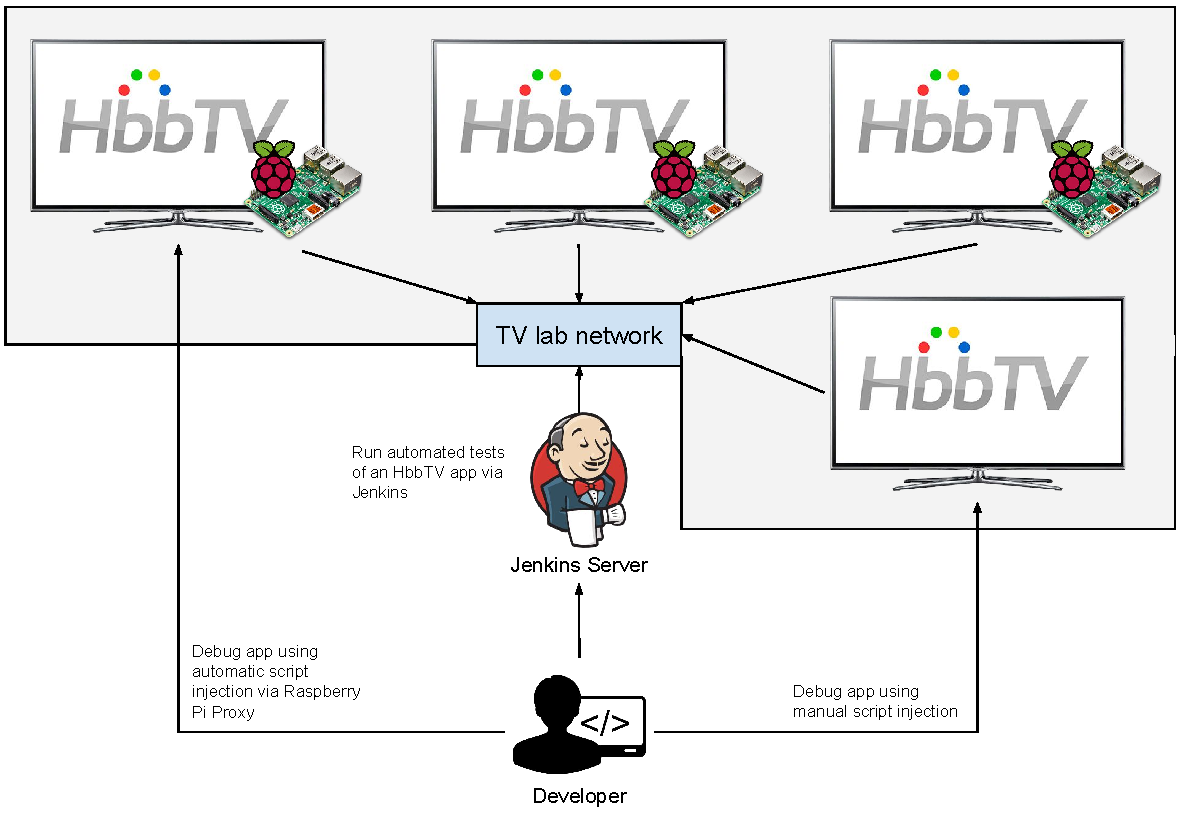
\includegraphics[width=15cm]{big_picture.pdf}
  \caption{Big picture of how developers will be able to develop and test their HbbTV application}\label{fig:bigpicture}
\end{figure}

With both platforms in place the developer of an HbbTV app will be able to debug and test his applications
with modern tooling that is used in today's web development. Since the technologies for both is based on
common used and well-defined standards we don't restrict our self to another homegrown solution instead we
allow the integration to other tooling which makes us less bound to a certain tool. As described in figure
\ref{fig:bigpicture} the developer will have three different ways to utilize the TV. One way is to use
a TV that was equipped with a Raspberry Pi running the automation driver on it. The Pi will act as a proxy
and allows to automatically inject the automation script as well as track network data to display requests
and responses made by the HbbTV application in the DevTools app. Because of the amount of edge cases and
issues this proxy can run into, there will be no guarantee that this approach is bullet proof and easy to
use. Running this kind of setup requires some amount of effort to maintain it. That's why there will be
another way to debug and test HbbTV apps without a Raspberry PI. This solution will require some manual
changes to the source code of the app to make it work.

\section{Outline\label{sec:outline}}

Before we jump into the details of how all this will be implemented we will first look at some fundamentals
of the technology that will be used. Next to the HbbTV standard, its market support and distribution as well
as how developers build HbbTV apps these days, there will be a section on the WebDriver protocol and how
automated testing changed the industry from moving from waterfall to an agile methodology thanks to
continuous integration and delivery. In the next chapter we define the requirements and find out what is
needed to solve the issues that are mentioned in the motivation section. Once we have that we can define
our concept where all components of the created tool are described in detail with explanation on how they
interact and work with each other. It will also outline how Appium works and how this tool fits into
Appiums Ecosystem. In the implementation part of this thesis we then go into more detail on how certain
parts are build and which technology is behind it. It will explain how certain components have to be
setup as well as how you need to configure all network components to create your own TV grid. At the
end we conduct an evaluation of a similar product that tries to solve almost the same problem in a
different way before we end up with a summary of the work, giving an outlook about future work and
interesting features that could be implemented next.
